\documentclass[a4paper,french]{paper}
\usepackage{../../_latex_assets/villemejane_iogs_ceti}

%Informations about this document 
%------------------------------------------
\def\module{Conception Electronique pour le Traitement de l'Information}
\def\moduleAbrege{5N-027-SCI / CéTI}
\def\annee{}

\def\titre{Bloc 1 / Capteurs et mise en forme}
\author{Julien VILLEMEJANE}

\subtitle{Bloc 1}
\institution{LEnsE / Institut d'Optique Graduate School}

\title{\titre}
\begin{document} 
%Beginning First Page. 
%------------------------------------------
\enteteThematiqueObligatoire{}

%Beginning Content. 
%------------------------------------------

%%%%%%%%%%%%%%%%%%%
\encadreTDExo{1 - Abaisser une tension}{
Proposer un circuit permettant d'abaisser une tension d'un facteur $k$.

$0 < k < 1$ 
}

%%%%%%%%%%%%%%%%%%%
\encadreTDExo{2 - Élever une tension}{
Proposer un circuit permettant d'élever une tension d'un facteur $k$.

$k > 1$
}

%%%%%%%%%%%%%%%%%%%
\encadreTDExo{3 - Limiter une tension}{
Rappeler le fonctionnement d'une diode.

Décrire le fonctionnement du montage suivant :

\begin{center}
	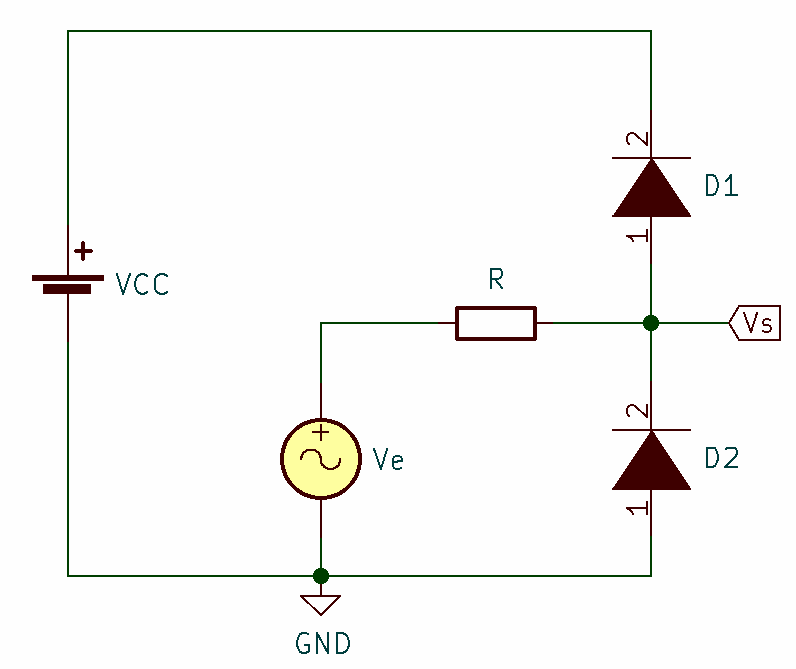
\includegraphics[width=6cm]{images/limiteur_diode.png}
\end{center}

}

%%%%%%%%%%%%%%%%%%%
\encadreTDExo{4 - Amplifier un signal}{
Proposer un circuit permettant d'amplifier un signal de $27dB$, tout en garantissant une bande-passante de $400 kHz$.

On utilisera des amplificateurs linéaires intégrés de type TL081 (documentation partielle donnée en annexe).
}


%%%%%%%%%%%%%%%%%%%
\encadreTDExo{5 - Additionner des signaux}{
On se propose d'étudier le circuit suivant :
\begin{center}
	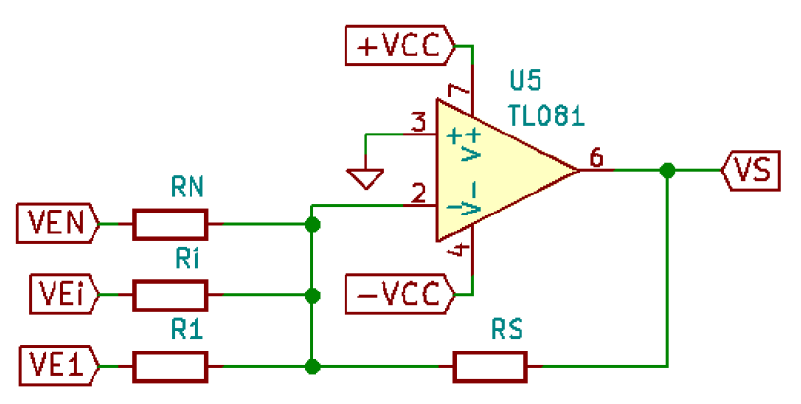
\includegraphics[width=10cm]{images/ali_ampli_somme.png}
\end{center}
}


%%%%%%%%%%%%%%%%%%%
\encadreTDExo{6 - Mettre en forme un capteur de température}{
On se propose d'étudier le circuit suivant :

\begin{center}
	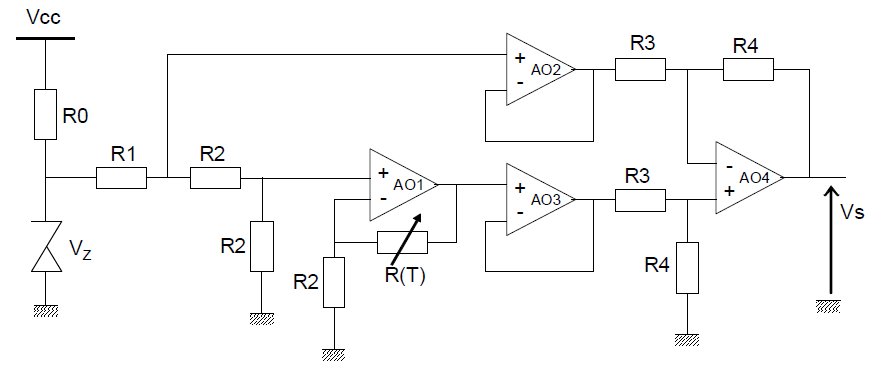
\includegraphics[width=16cm]{images/capteur_conditionnement.png}
\end{center}

La thermistance utilisée est de type PT100. La relation entre sa résistance (en Ohms) et la température (en \degre{}C) est la suivante :
$$R(T) = 100~(1 + 3.908×10^{-3} T - 5.802×10^{-7} T^2)$$

}

\end {document}